% !TeX root = Bericht.tex
% !TeX spellcheck = de_DE
\section{Experimental setup and procedure}
Before the actual measuring started, we discussed the safety aspects of working with a laser. Therefore, we dismounted all jewelry and wristwatches to minimize the risk of reflecting the laser in an unwanted direction. After this, we took a look at the mounted optical components and checked if the mirrors were in the correct position, as well as whether the collimation was well-adjusted to get a precise output beam. We used a \ch{HeNe} Laser with a wavelength of $\lambda = 632.8 \unit{nm}$. After these steps, we switched off the laser to safely measure the distance between the mirrors and the AOM, as well as the point where we will later measure the distance between the \nth{0} and \nth{1} order diffracted beams. This measurement was taken with a measuring tape with estimated errors of $ \pm 0.2 \unit{cm} $ for the first two lengths and $ \pm 0.1 \unit{cm} $ for the third length, as we have a very solid measuring point at the end of the beam (actual lengths in \autoref{fig:setup}).

Since we are using an amplifier to increase the signals strength, we have to take the amps gain into consideration when setting the signals amplitude on the frequency generator. From the datasheet (see \autocite{DatenBlattAmplifier}), we found that the amplifier boosts the signal by $33 \unit{dB}$, which corresponds to an input power increase by a factor of 2000. In order to put $2 \unit{W}$ through the AOM (this is the maximum power) we have to set the function generator to $1 \unit{mW}$. This corresponds to a peak-to-peak voltage of $632 \unit{mVpp}$ \autocite{UmrechnungsTabelleDB}. The frequency generator, where we can adjust these parameters, is shown in \autoref{fig:Frequnezgenerator}. 

Following this, we initiated the laser and commenced the process of identifying both the \nth{1} and \nth{0} orders of the diffracted beam. The input parameters for the AOM were configured to $500 \unit{mW}$ and $80 \unit{MHz}$. With this setup, we accurately determined the Bragg angle by maximizing the power of the \nth{1} order beam by adjusting the rotation mount. Measurements of the mentioned distances were conducted using a measuring tape. The corresponding setup is visually depicted in \autoref{fig:setup}.
\begin{figure}[H]
	\centering
	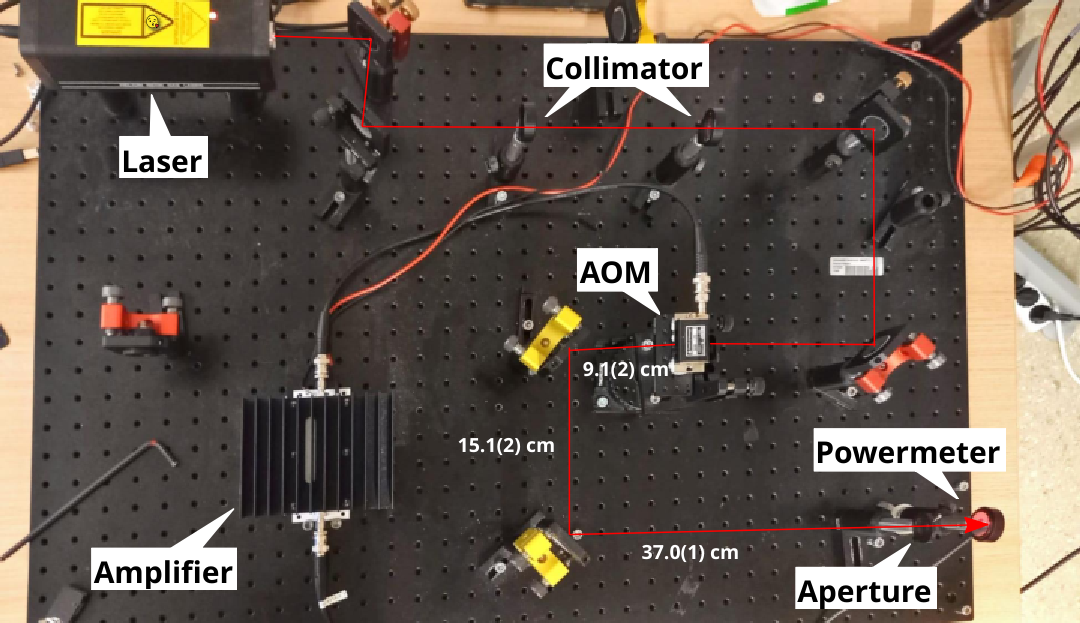
\includegraphics[width=\textwidth]{aufbau}
	\caption{A picture of the experimental setup. The path of the laser beam is traced from the laser in the top left corner to the power meter on the bottom right. All the major components are labeled accordingly. The measured path length from the Acousto-optical Module (AOM) to the power meter is also given.}
	\label{fig:setup}
\end{figure}
Afterwards, we measured the power before and after the AOM without a modulation signal to assess the internal losses ($IL$). Proceeding, the power of the AOM was varied from $0 \unit{W}$ to $2 \unit{W}$, with the corresponding $\oldunit{mVpp}$ as mentioned above. Opting for $30 \unit{mVpp}$ steps, we measured the power of the \nth{0} and the \nth{1} orders to assess $\varepsilon$, thereby positioning ourselves to fit a function referenced in \autoref{subsec:AOM} to determine the saturation power $\P{sat}$.

In the next step, the intention was to determine the frequency dependence of the AOM. Therefore, the power was set to $500 \unit{mW}$, and the frequency was modulated in the range of $60 - 100 \unit{MHz}$ in $3 \unit{MHz}$ steps (The last two steps were $2 \unit{MHz}$ each to precisely reach $100 \unit{MHz}$). The power of the \nth{1} order was measured, as well as the distance between the \nth{0} and \nth{1} order beam. With this length, we are able to determine the Bragg angle. To obtain a more accurate result, the measurement was taken at a larger distance (by projecting the beams onto a wall). The length after the \nth{2} mirror after the AOM ($37.0(1) \unit{cm}$ so far) was extended to $140.0(2) \unit{cm}$.

\begin{figure}[H]
	\centering
	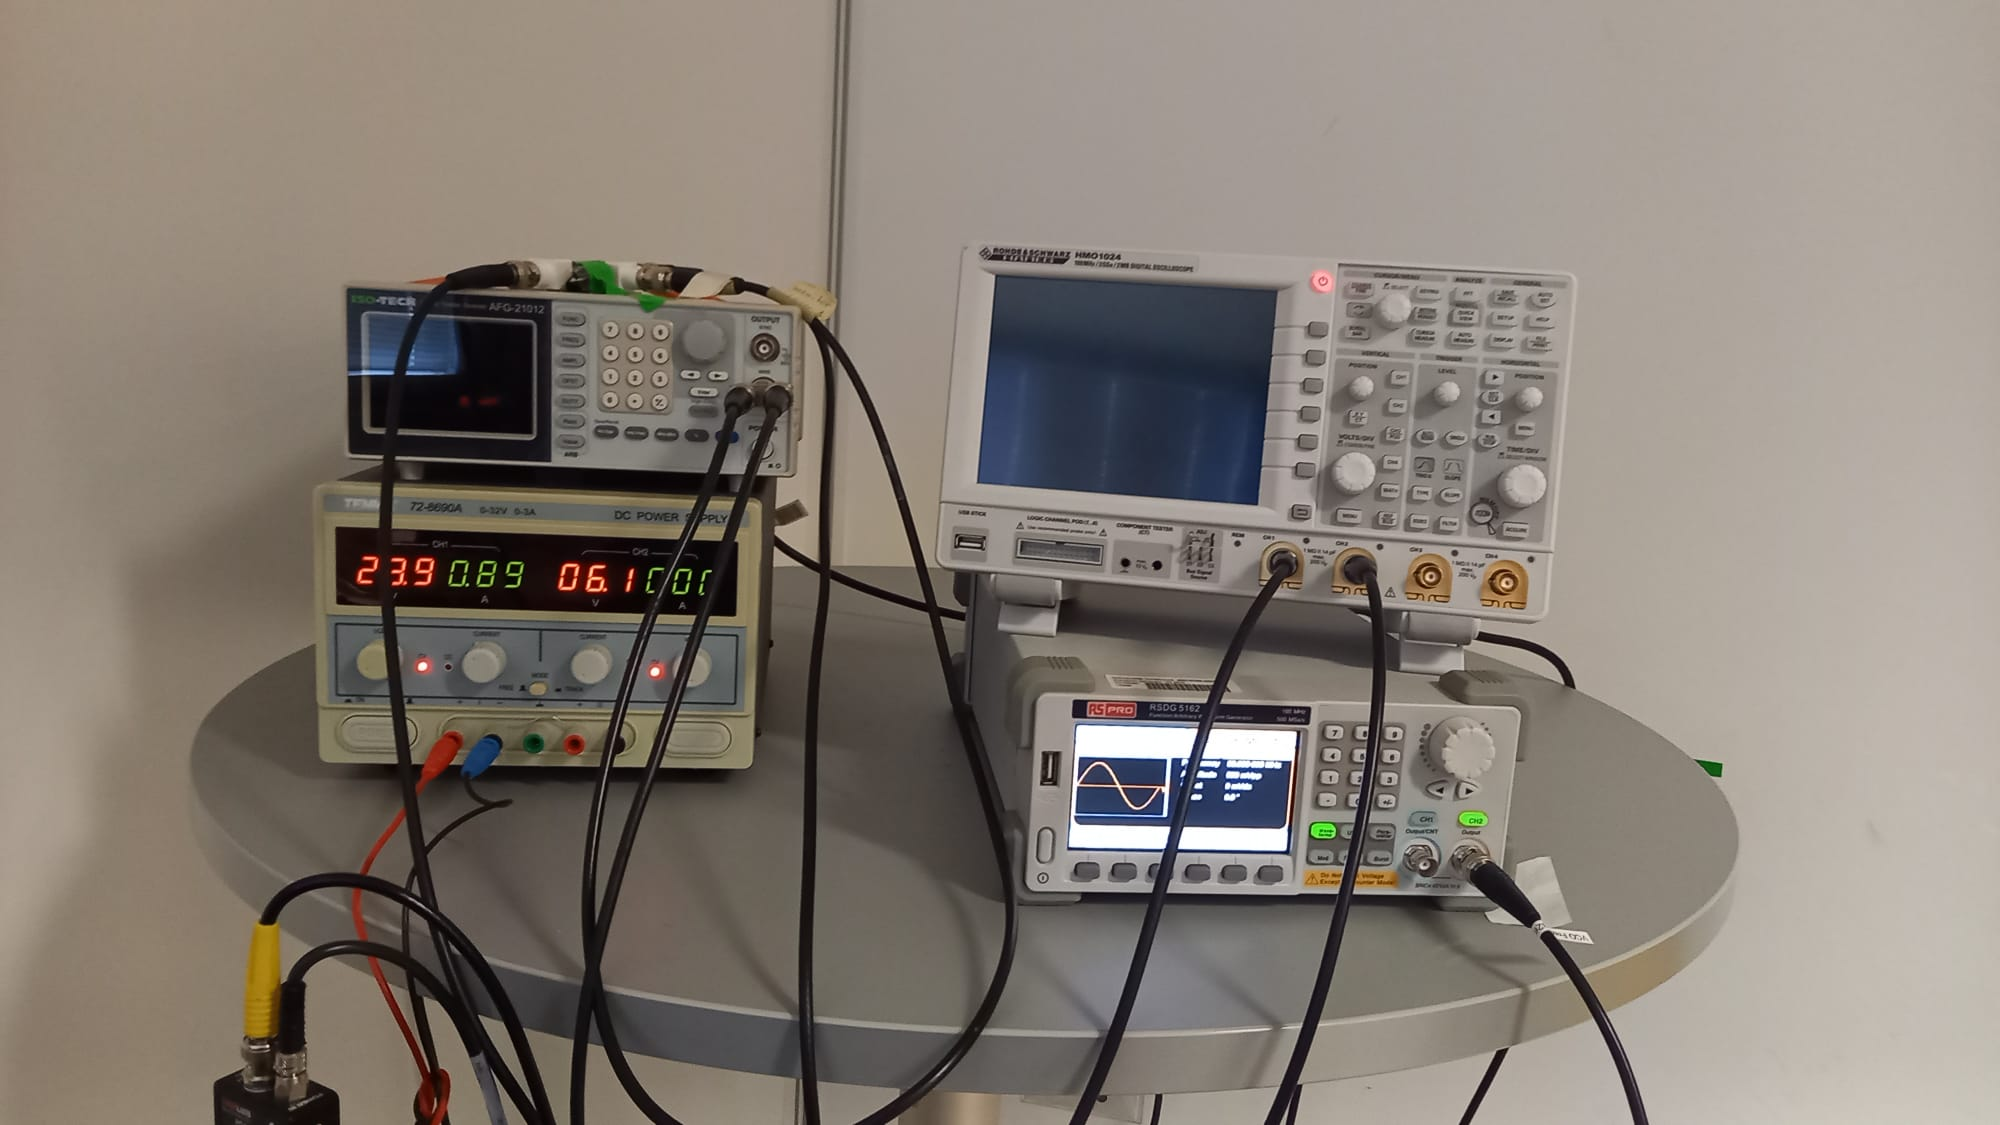
\includegraphics[width=\textwidth]{Bild_Frequenzgenerator}
	\caption{This figure shows a picture of the power supply for the amplifier (on the left) as well as the frequency generator (on the right), where it is possible to set the $\oldunit{mVpp}$ and the frequency.}
	\label{fig:Frequnezgenerator}
\end{figure}

Thereafter, the focus shifted to the angular dependence of the AOM in perspective to the quality factor $Q$. We began by determining the deadzone of the rotation mount, as well as verifying the gear ratio provided in \autocite{Drehtisch}. For the deadzone, we estimate it to be 5 ticks, and we verified the gear ratio to be 1/25 (25 ticks on the screw are equal to \ang{1}). Now the task was to evaluate the power at the \nth{1} order beam for angles between -\ang{1} and \ang{1} with the AOM parameters of $80 \unit{MHz}$ and $500 \unit{mW}$. Here we decided to use a step size of 3 ticks in the outer range, and as we got closer to \ang{0}, we made finer steps with 2 ticks. Surprisingly, the maximum value was not at \ang{0}, so we decided to take more values in the positive angular direction to achieve a symmetric measuring range around the maximum value. To minimize measurement errors from the screws deadzone all measurements were made by continuously adjusting the screw from the same direction. 

Finally, the task was to analyze the angular dependence of the maximum diffraction efficiency. Therefore, we set the power of the AOM to $500 \unit{mW}$ and then changed the frequency in the range of $60 - 100 \unit{MHz}$, using $5 \unit{MHz}$ steps. At each frequency, we aimed to maximize the power of the \nth{1} order by adjusting the angle of the rotation mount and recording the power.



